\section{\Large PROBLEM SET 3}
\subsection{PROBLEM 1}
\textit{Impose that satellite is axial-symmetric (Ix$=$Iy$\neq$Iz). Repeat numerical simulation from previous pset using initial condition 4) from previous pset.}

Problem 1 was solved by setting $I_{x} = I_{y} = \qty{7707.07}{kg \cdot m^2}$ and using the same Euler equation solver from Problem Set 2, Problem 5 with the same initial conditions ($\omega_{x} = \qty{8}{\degree\per\second}$, $\omega_{y} = \qty{4}{\degree\per\second}$).

\begin{figure}[H]
\centering
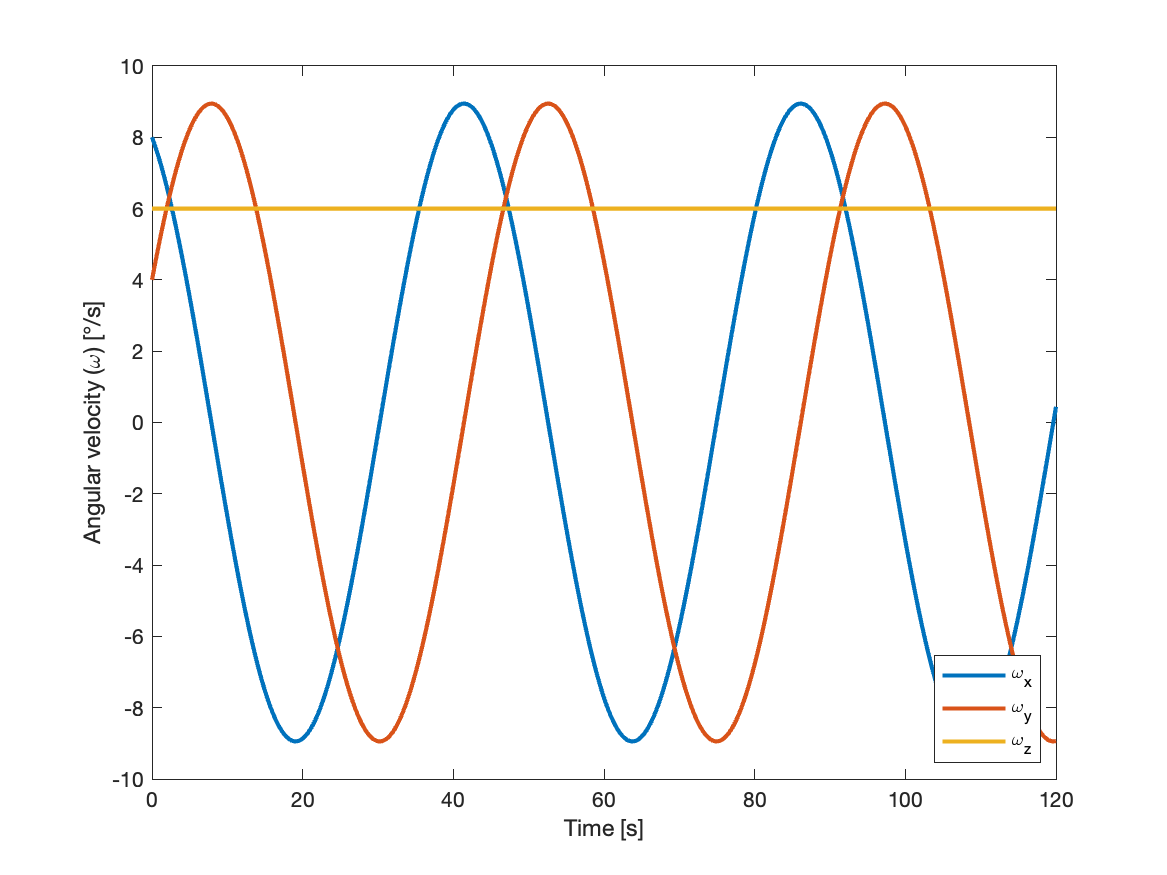
\includegraphics[scale=0.6]{Images/ps3_problem1.png}
\caption{Numerical solution results}
\label{fig:ps3_problem1}
\end{figure}


\subsection{PROBLEM 2}
\textit{Program analytical solution for axial-symmetric satellite. Compute it at same time steps and from same initial conditions.}

The analytical solution to the Euler equations for an axial-symmetric satellite is based on variables $\lambda$ and $\omega_{xy}$, as defined below.
\begin{align*}
    \lambda = \frac{I_{z} - I_{x}}{I_{x}} \omega_{z_{0}} \\
    \omega_{xy} = (\omega_{x_{0}} + i \omega_{y_{0}}) e^{i \lambda t}
\end{align*}

We take the real and imaginary parts of this result to obtain an analytical solution.
\begin{align*}
    \omega_x = \text{Re}(\omega_{xy}) \\
    \omega_y = \text{Im}(\omega_{xy}) \\ 
    \omega_z = \omega_{z_{0}}
\end{align*}


\begin{figure}[H]
\centering
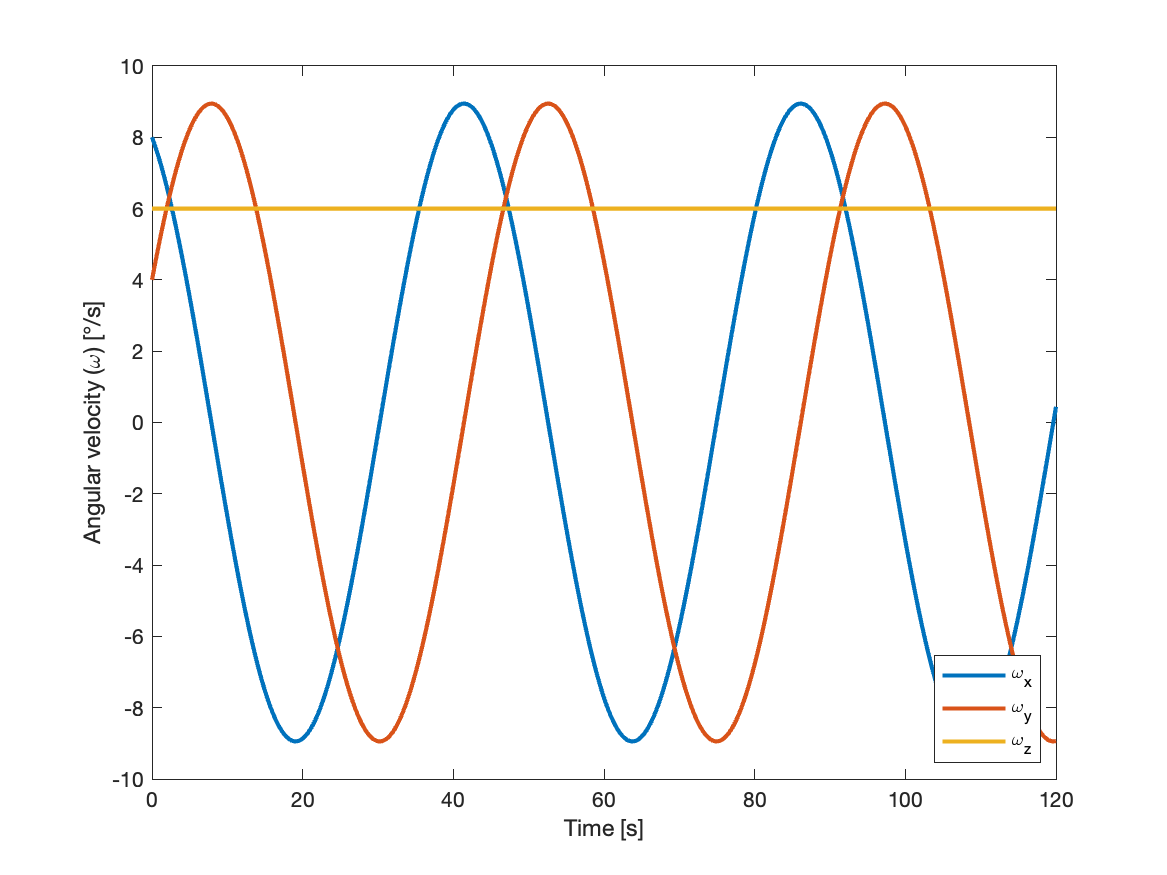
\includegraphics[scale=0.6]{Images/ps3_problem2.png}
\caption{Analytical solution results}
\label{fig:ps3_problem2}
\end{figure}


\subsection{PROBLEM 3}
\textit{Compare numerical and analytical solutions. Plot differences (errors), do not only superimpose absolute values. Tune numerical integrator for large discrepancies. Are angular velocity vector and angular momentum vector changing according to theory in principal axes?}

Figure \ref{fig:ps3_problem3} is the error between the numerical and analytical solutions. The angular velocity vector and angular momentum vectors rotate at a constant angle from the z-axis along a rotating plane, as observed in Figure \ref{fig:Body Axis Momentum Snapshots}. This matches the expected theoretical behavior.

\begin{figure}[H]
\centering
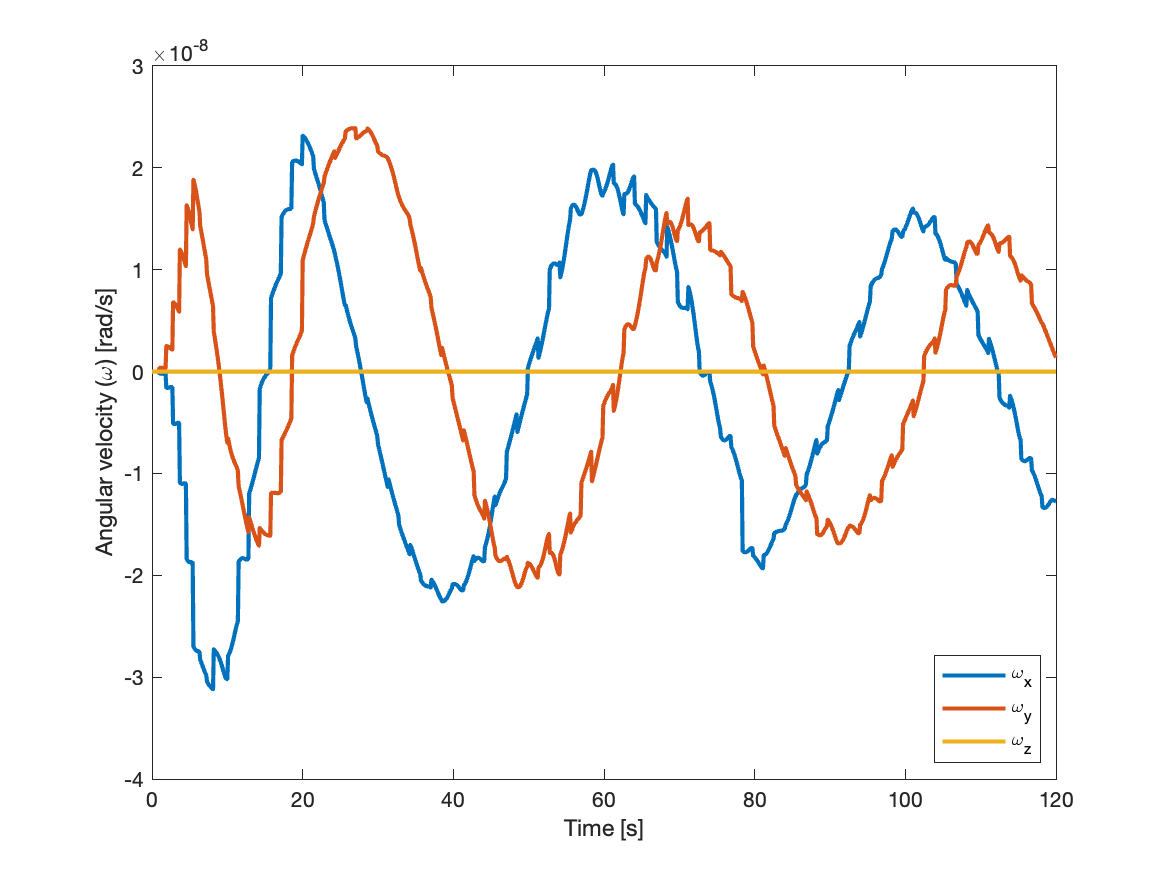
\includegraphics[scale=0.6]{Images/ps3_problem3.png}
\caption{Error between numerical and analytical solutions}
\label{fig:ps3_problem3}
\end{figure}

\begin{figure}[H]
  \centering
  \begin{tabular}{@{}c@{}}
  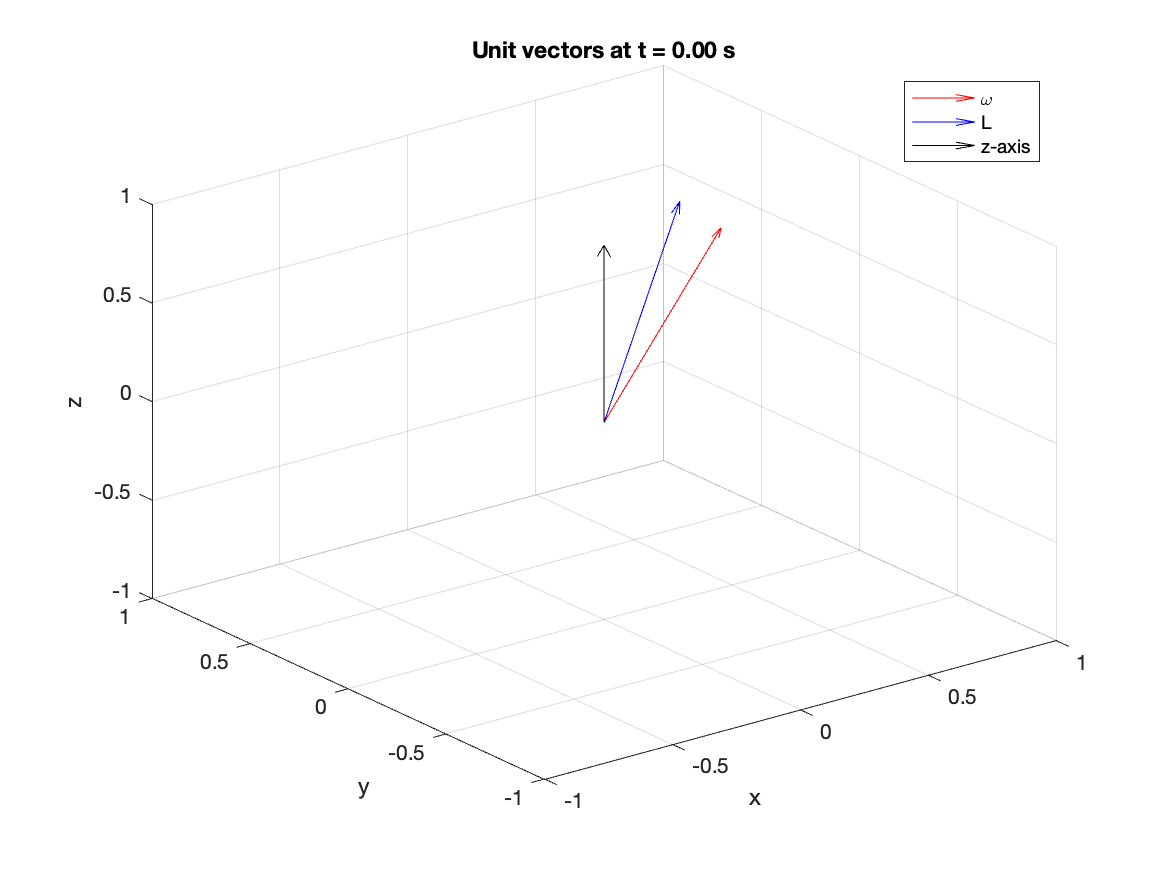
\includegraphics[width=.47\linewidth]{Images/ps3_problem3_vectors_1.png}
  \end{tabular}
  \begin{tabular}{@{}c@{}}
  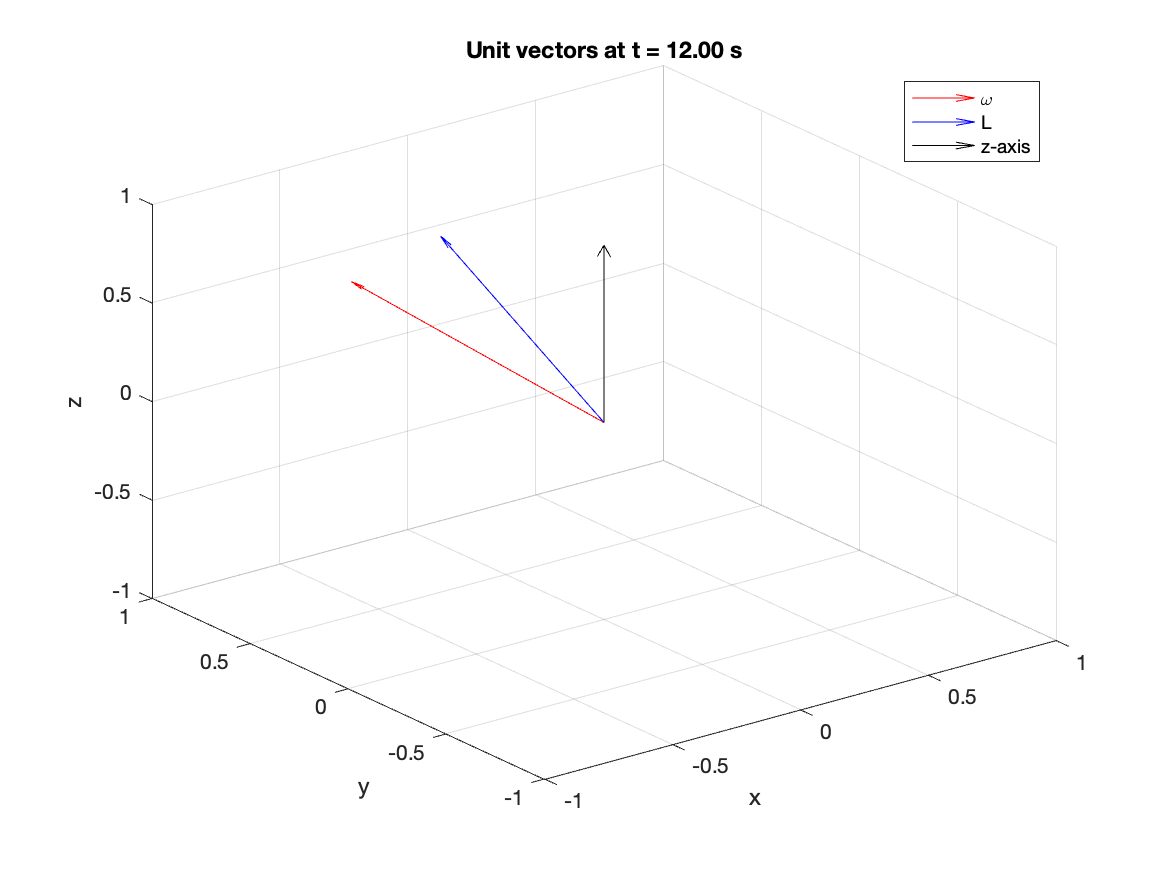
\includegraphics[width=.47\linewidth]{Images/ps3_problem3_vectors_121.png}
  \end{tabular}
  \begin{tabular}{@{}c@{}}
  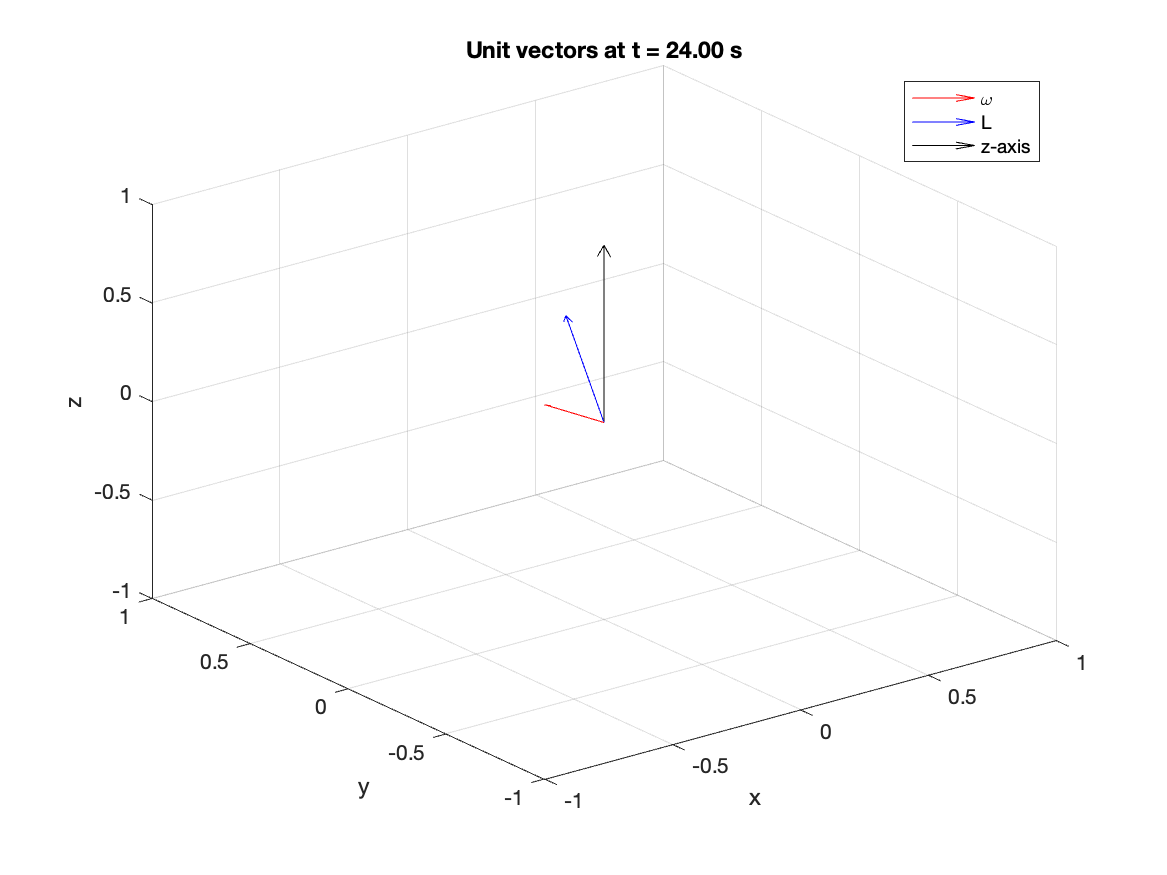
\includegraphics[width=.47\linewidth]{Images/ps3_problem3_vectors_241.png}
  \end{tabular}
  \begin{tabular}{@{}c@{}}
  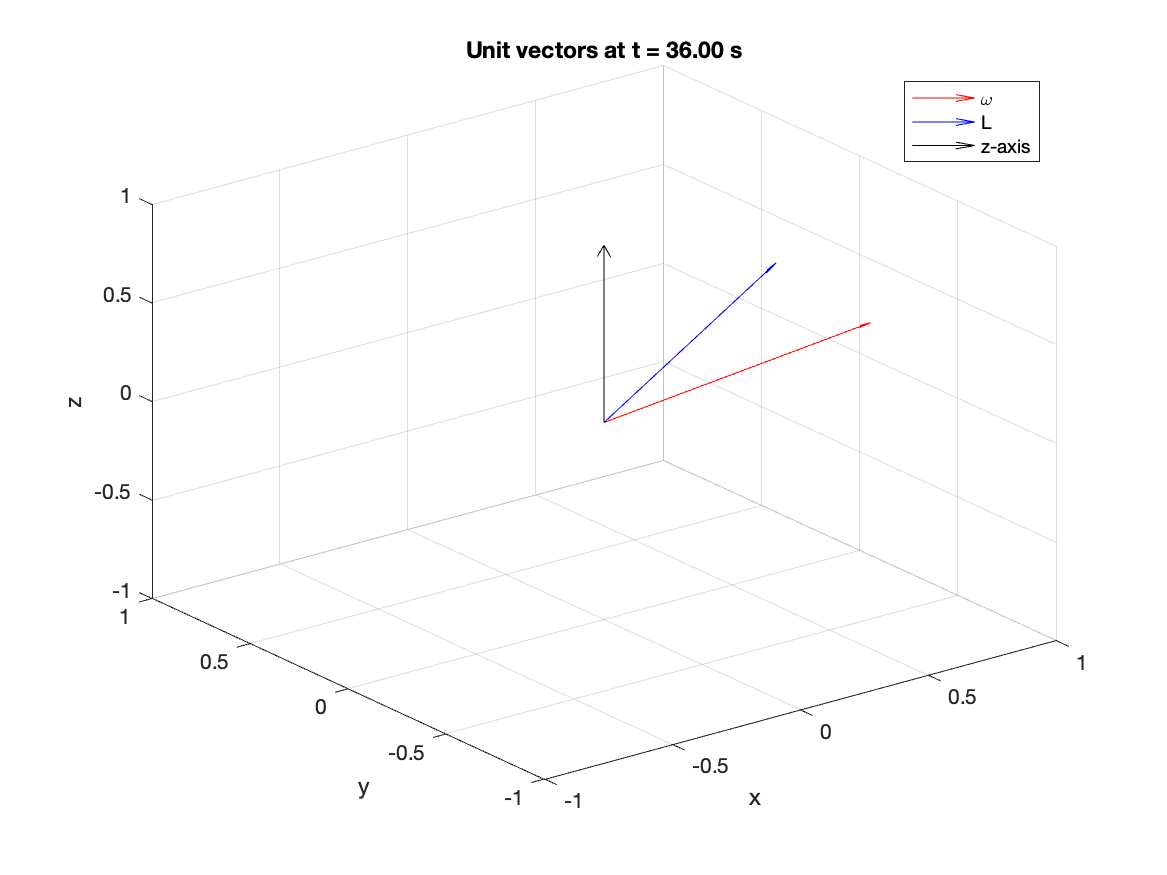
\includegraphics[width=.47\linewidth]{Images/ps3_problem3_vectors_361.png}
  \end{tabular}
  \caption{Unit vectors for angular velocity (red) and angular momentum (blue) at t = 0s, 12s, 24s, 36s.}
  \label{fig:Body Axis Momentum Snapshots}
\end{figure}


\subsection{PROBLEM 4}
\textit{Program Kinematic equations of motion correspondent to a nominal attitude parameterization of your choice.}

We choose a nominal attitude parameterization of quaternions, our choice being based on the absence of singularities. The following function computes the time derivative for a state consisting of quaternions (4 parameters) and angular velocity (3 parameters).

The equations below describe the propagation of kinematics using quaternions.

\begin{align*}
\Vec{\Omega} &= 
    \begin{bmatrix}
    0 & \omega_{z} & -\omega_{y} & \omega_{x}\\
    -\omega_{z} & 0 & \omega_{x} & \omega_{y}\\
    \omega_{y} & -\omega_{x} & 0 & \omega_{z}\\
    -\omega_{x} & -\omega_{y} & -\omega_{z} & 0
    \end{bmatrix}\\
\frac{d \Vec{q}}{dt} &= \frac{1}{2} \Vec{\Omega} \Vec{q}(t)
\end{align*}

\lstinputlisting{src/kinQuaternion.m}

We can use the previous function to perform a forward Euler numerical integration. We call the previous function over a fixed time step to compute the evolution of the state.

\lstinputlisting{src/kinQuaternionForwardEuler.m}

For improved precision, we implement a 4th order Runge-Kutta method, which uses a weighted sum of slopes to obtain a better result. This also calls the time derivative function, but does so with different values of the state, which are weighted to obtain the next state for each step.

\lstinputlisting{src/kinQuaternionRK4.m}


\subsection{PROBLEM 5}
\textit{Program Kinematic equations of motion correspondent to a different attitude parameterization from the previous step. This is used for comparison, to get familiar with different approaches, and as fall back solution in the case of singularities.}

Similarly, we create a function that computes the time derivative of a state consisting of Euler angles and angular velocity.

The equations for the propagation of kinematics for Euler angles is below.

\begin{align*}
\frac{d \phi}{dt} &= \frac{\omega_{x} \sin(\psi) + \omega_{y} \cos(\psi)}{\sin(\theta)}\\
\frac{d \theta}{dt} &= \omega_{x} \cos(\psi) - \omega_{y} \sin(\psi)\\
\frac{d \psi}{dt} &= \omega_{z} - (\omega_{x} \sin(\psi) + \omega_{y} \cos(\psi)) cot(\theta)
\end{align*}

\lstinputlisting{src/kinEulerAngle.m}

We can propagate this with forward Euler, as in the previous section.

\lstinputlisting{src/kinEulerAngleForwardEuler.m}

For our actual implementation, we choose to use the time derivative function with \texttt{ode113} for improved accuracy. Note that while this is possible with the Euler angle time derivative, it cannot be done as simply for quaternions, as they require normalization at each step, hence our decision to implement RK4.


\subsection{PROBLEM 6}
\textit{Numerically integrate Euler AND Kinematic equations from arbitrary initial conditions (warning: stay far from singularity of adopted parameterization). Multiple revolutions. The output is the evolution of the attitude parameters over time. These attitude parameters describe orientation of principal axes relative to inertial axes.}

We integrate our attitude parameterizations (including angular velocity using Euler equations–see previous section for numerical integration state) over 600 seconds. Notice that since we have no external torques, our attitude parameters vary periodically.

\begin{figure}[H]
\centering
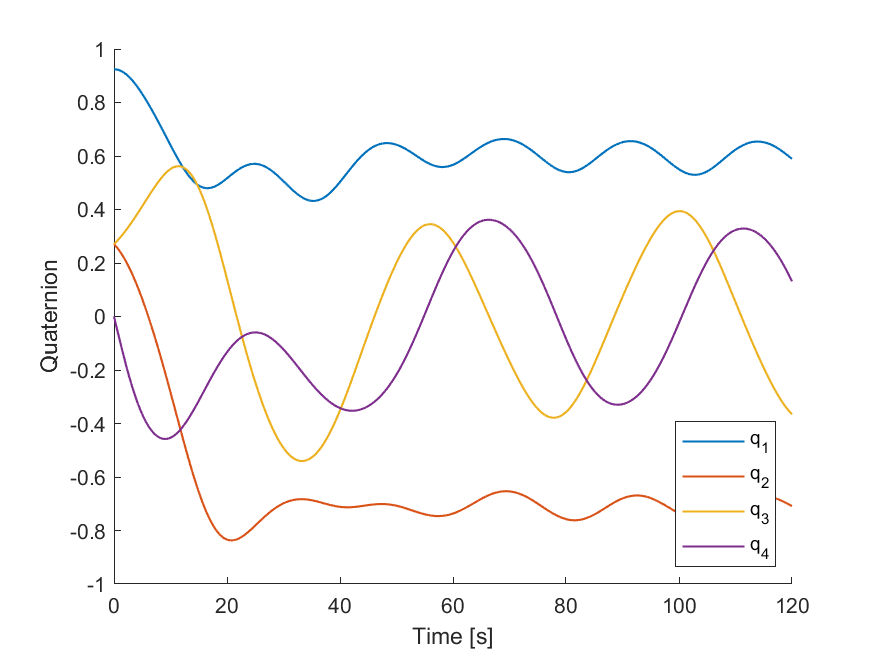
\includegraphics[scale=0.6]{Images/ps3_problem6_quaternions.png}
\caption{Evolution of quaternions}
\label{fig:ps3_problem6_quaternions}
\end{figure}

\begin{figure}[H]
\centering
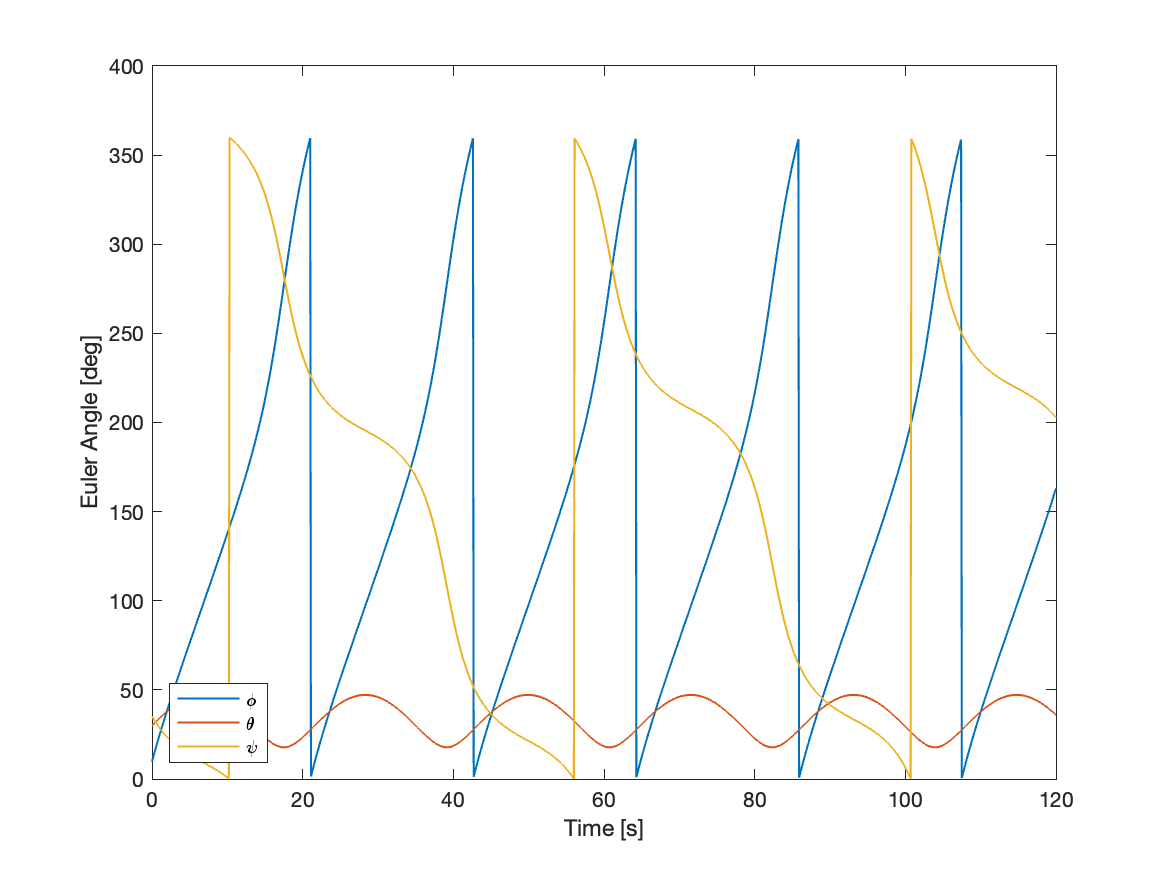
\includegraphics[scale=0.6]{Images/ps3_problem6_euler.png}
\caption{Evolution of Euler angles}
\label{fig:ps3_problem6_euler}
\end{figure}

\subsection{PROBLEM 7}
\textit{Since inertial position, velocity, and attitude, are known at the same time throughout the simulation, it is now possible to express vectors in the reference systems of interest.}

\textit{a. Compute angular momentum vector in inertial coordinates and verify that it is constant (not only its magnitude as in PS2) by plotting its components.}

Figure \ref{fig:ps3_problem7a} shows the components of the angular momentum vector over time. As expected, the angular momentum vector (and its individual components) all remain constant in the absence of external torques.

\begin{figure}[H]
\centering
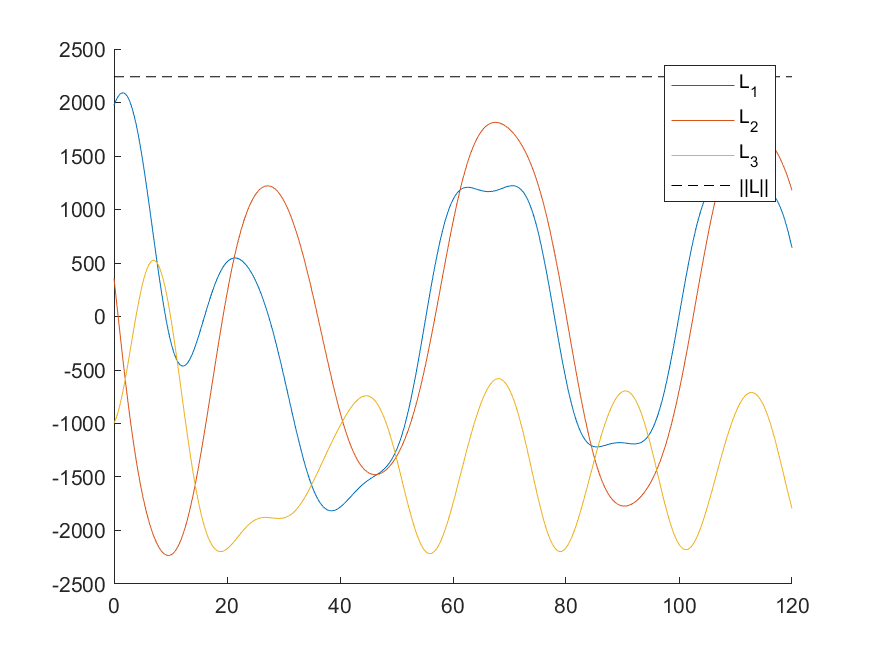
\includegraphics[scale=0.6]{Images/ps3_problem7a.png}
\caption{Angular momentum in inertial coordinates is constant}
\label{fig:ps3_problem7a}
\end{figure}

\textit{b. Compute angular velocity vector in inertial coordinates and plot the herpolhode in 3D (line drawn in inertial space by angular velocity). Is the herpolhode contained in a plane perpendicular to the angular momentum vector? Show it.}

Figure \ref{fig:ps3_problem7b} shows the angular momentum and angular velocity vectors overlaid with the herpolhode. The animation (see caption) shows the evolution of the herpolhode and provides a better visualization of the herpolhode's orientation in a plane perpendicular to the angular momentum vector. 

\begin{figure}[H]
\centering
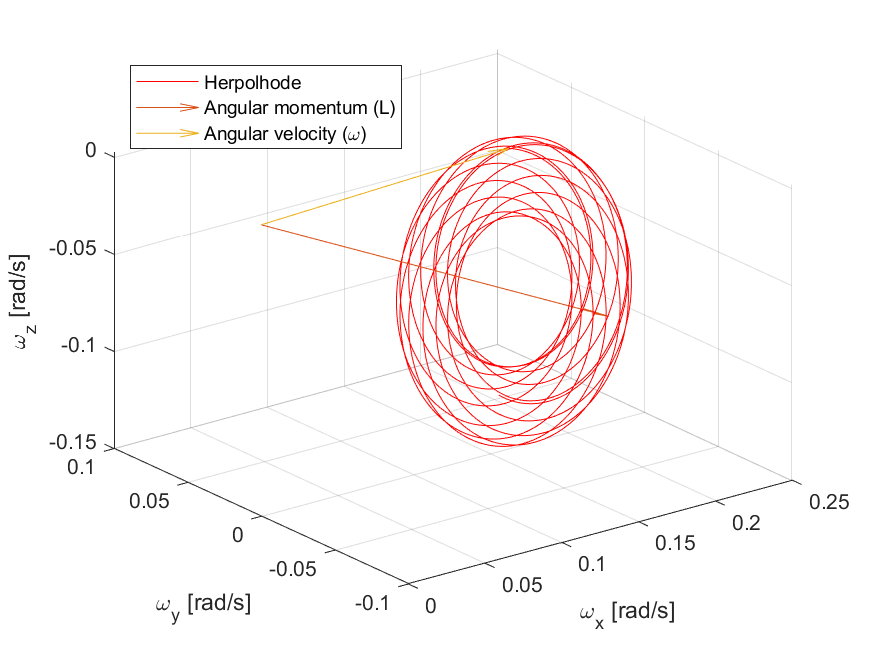
\includegraphics[scale=0.6]{Images/ps3_problem7b.png}
\caption{Herpolhode (Animated: \protect\url{https://tinyurl.com/herpolhode})}
\label{fig:ps3_problem7b}
\end{figure}

\textit{c. Compute and plots unit vectors of orbital frame, body axes, and principal axes in 3D as a function of time in inertial coordinates. (Be creative on how to show moving vectors in 3D).}

Figures \ref{fig:ps3_problem7c_rtn}, \ref{fig:ps3_problem7c_body}, and \ref{fig:ps3_problem7c_principal} include the plots of the orbital, body, and principal axes over the course of a single orbit.

\begin{figure}[H]
\centering
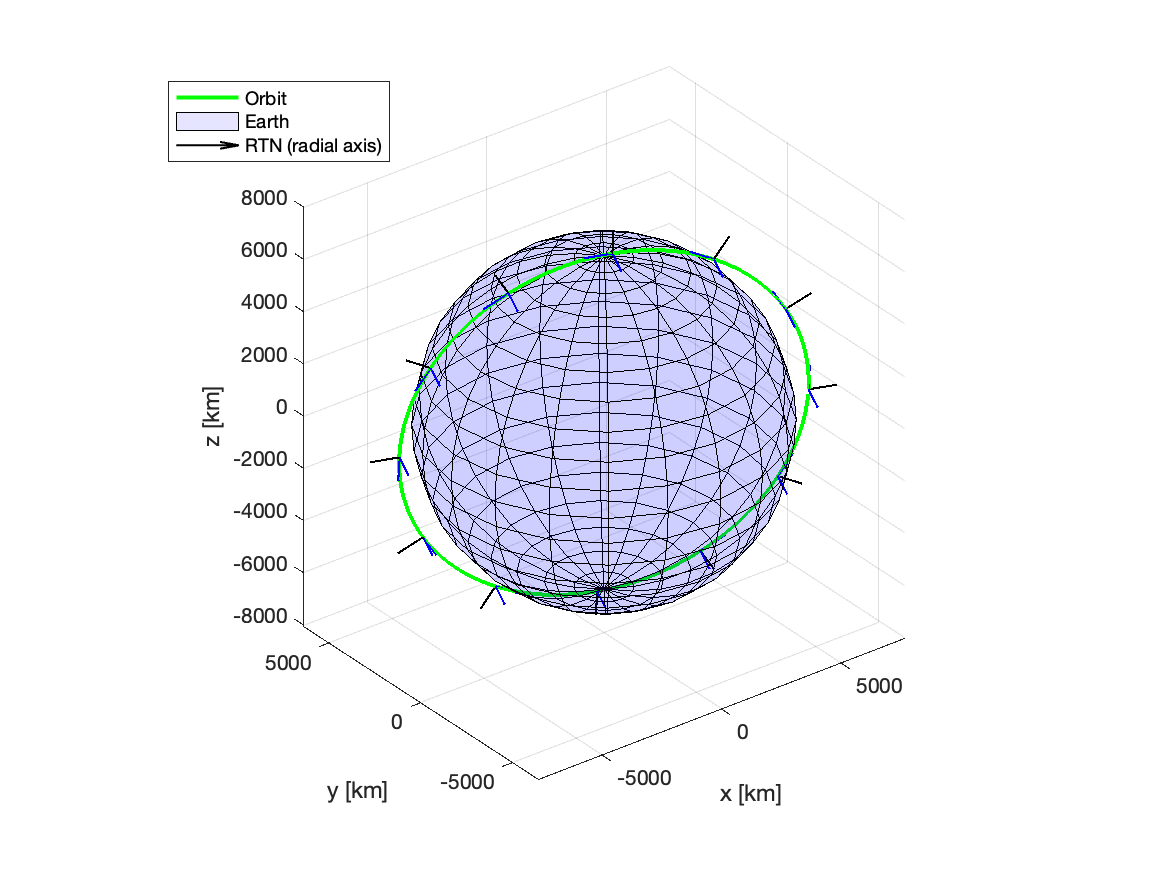
\includegraphics[scale=0.6]{Images/ps3_problem7c_rtn.png}
\caption{Propagation of RTN frame}
\label{fig:ps3_problem7c_rtn}
\end{figure}

\begin{figure}[H]
\centering
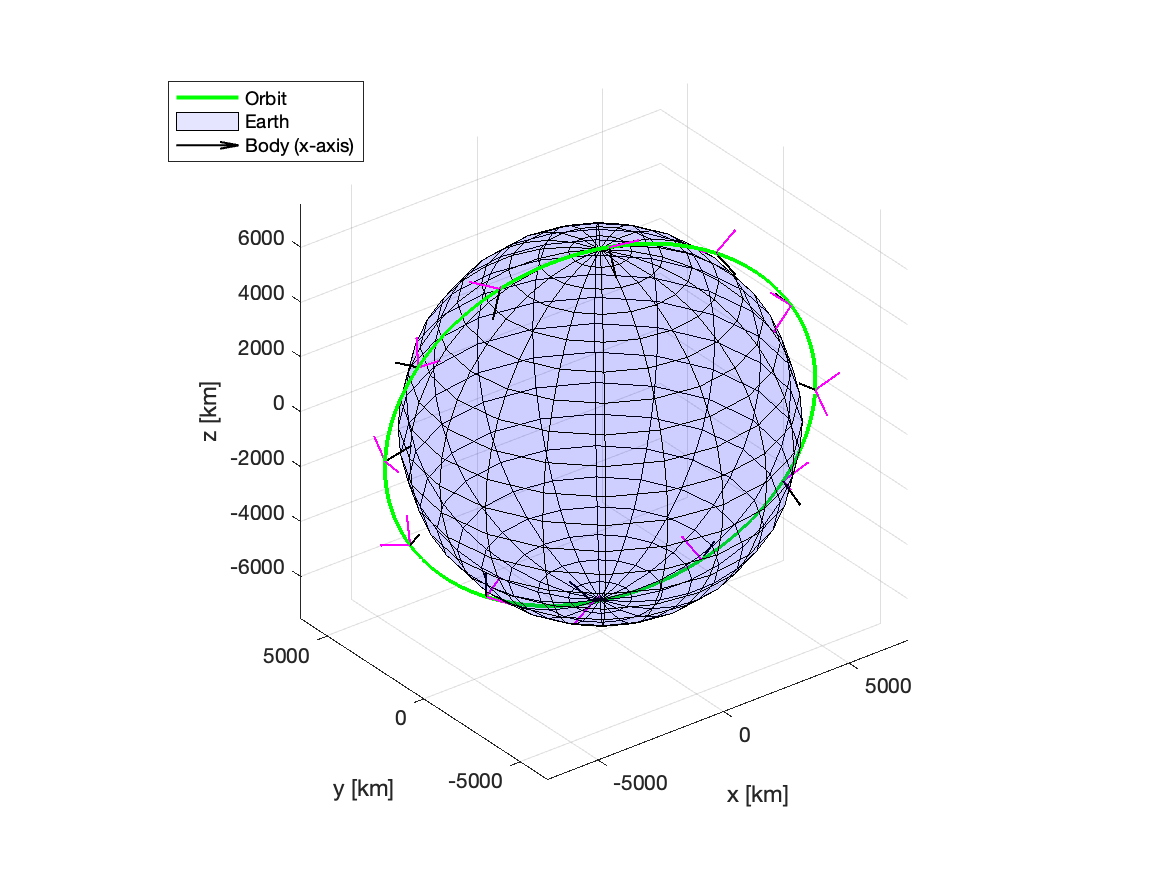
\includegraphics[scale=0.6]{Images/ps3_problem7c_body.png}
\caption{Propagation of body axes}
\label{fig:ps3_problem7c_body}
\end{figure}

\begin{figure}[H]
\centering
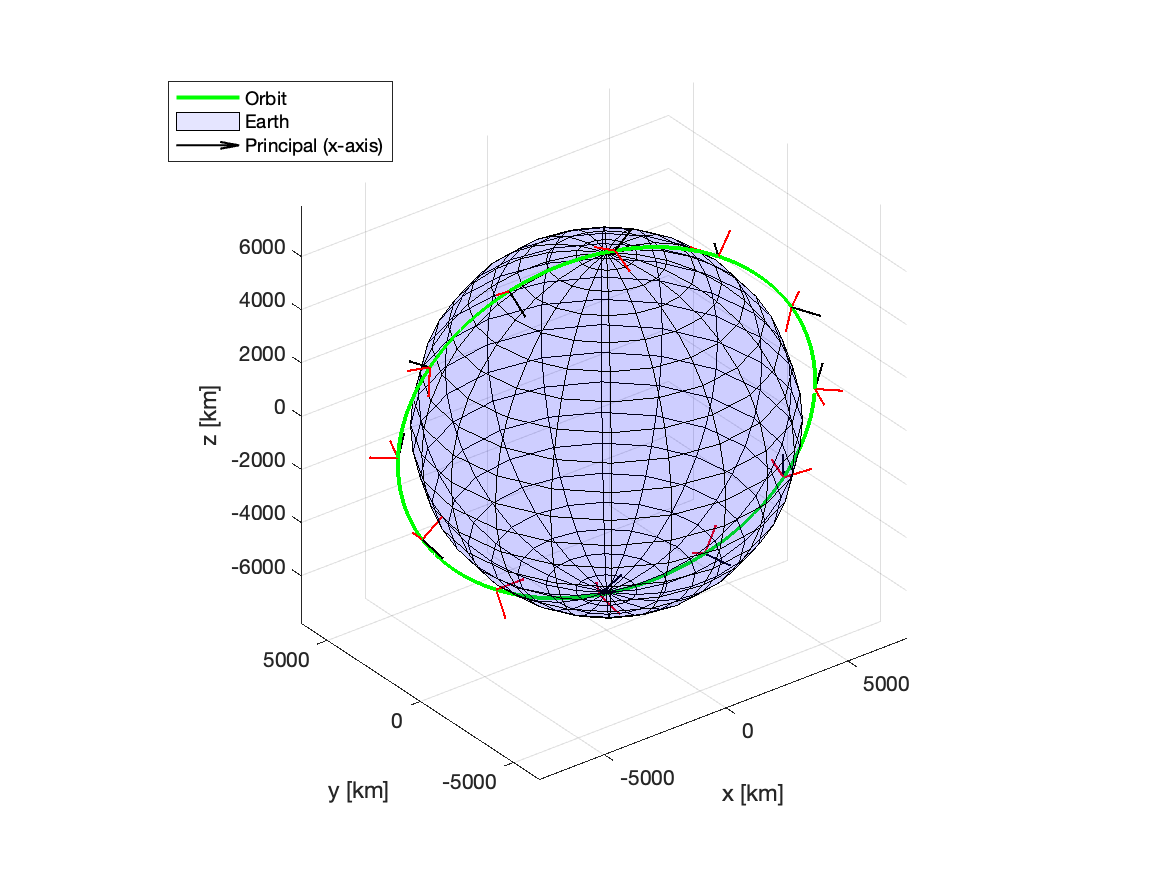
\includegraphics[scale=0.6]{Images/ps3_problem7c_principal.png}
\caption{Propagation of principal axes}
\label{fig:ps3_problem7c_principal}
\end{figure}